% This is "sig-alternate.tex" V2.1 April 2013
% This file should be compiled with V2.5 of "sig-alternate.cls" May 2012
%
% This example file demonstrates the use of the 'sig-alternate.cls'
% V2.5 LaTeX2e document class file. It is for those submitting
% articles to ACM Conference Proceedings WHO DO NOT WISH TO
% STRICTLY ADHERE TO THE SIGS (PUBS-BOARD-ENDORSED) STYLE.
% The 'sig-alternate.cls' file will produce a similar-looking,
% albeit, 'tighter' paper resulting in, invariably, fewer pages.
%
%--------------------------
% This .tex file (and associated .cls V2.5) produces:
%       1) The Permission Statement
%       2) The Conference (location) Info information
%       3) The Copyright Line with ACM data
%       4) NO page numbers
%
% as against the acm_proc_article-sp.cls file which
% DOES NOT produce 1) thru' 3) above.
%
% Using 'sig-alternate.cls' you have control, however, from within
% the source .tex file, over both the CopyrightYear
% (defaulted to 200X) and the ACM Copyright Data
% (defaulted to X-XXXXX-XX-X/XX/XX).
% e.g.
% \CopyrightYear{2007} will cause 2007 to appear in the copyright line.
% \crdata{0-12345-67-8/90/12} will cause 0-12345-67-8/90/12 to appear in the copyright line.
%
% ---------------------------------------------------------------------------
% This .tex source is an example which *does* use
% the .bib file (from which the .bbl file % is produced).
% REMEMBER HOWEVER: After having produced the .bbl file,
% and prior to final submission, you *NEED* to 'insert'
% your .bbl file into your source .tex file so as to provide
% ONE 'self-contained' source file.
%
% ================= IF YOU HAVE QUESTIONS =======================
% Questions regarding the SIGS styles, SIGS policies and
% procedures, Conferences etc. should be sent to
% Adrienne Griscti (griscti@acm.org)
%
% Technical questions _only_ to
% Gerald Murray (murray@hq.acm.org)
% ===============================================================
%
% For tracking purposes - this is V2.0 - May 2012

\documentclass{sig-alternate-05-2015}

%\usepackage{tabu}
%\usepackage{multirow}

\usepackage{booktabs}


\begin{document}

% Copyright
\setcopyright{acmcopyright}
%\setcopyright{acmlicensed}
%\setcopyright{rightsretained}
%\setcopyright{usgov}
%\setcopyright{usgovmixed}
%\setcopyright{cagov}
%\setcopyright{cagovmixed}

\clubpenalty=10000
\widowpenalty = 10000


%Conference
\conferenceinfo{GECCO'16,} {July 20-24, 2016, Denver, Colorado, USA.}

% \acmPrice{\$15.00}

%
% --- Author Metadata here ---
\CopyrightYear{2016} % Allows default copyright year (20XX) to be over-ridden - IF NEED BE.
\crdata{TBA}  % Allows default copyright data (0-89791-88-6/97/05) to be over-ridden - IF NEED BE.
% --- End of Author Metadata ---

\title{Parent Selection and Diversification in Genetic Programming}

%
% You need the command \numberofauthors to handle the 'placement
% and alignment' of the authors beneath the title.
%
% For aesthetic reasons, we recommend 'three authors at a time'
% i.e. three 'name/affiliation blocks' be placed beneath the title.
%
% NOTE: You are NOT restricted in how many 'rows' of
% "name/affiliations" may appear. We just ask that you restrict
% the number of 'columns' to three.
%
% Because of the available 'opening page real-estate'
% we ask you to refrain from putting more than six authors
% (two rows with three columns) beneath the article title.
% More than six makes the first-page appear very cluttered indeed.
%
% Use the \alignauthor commands to handle the names
% and affiliations for an 'aesthetic maximum' of six authors.
% Add names, affiliations, addresses for
% the seventh etc. author(s) as the argument for the
% \additionalauthors command.
% These 'additional authors' will be output/set for you
% without further effort on your part as the last section in
% the body of your article BEFORE References or any Appendices.

\numberofauthors{3} %  in this sample file, there are a *total*
% of EIGHT authors. SIX appear on the 'first-page' (for formatting
% reasons) and the remaining two appear in the \additionalauthors section.
%
\author{
% 1st. author
\alignauthor
Thomas Helmuth\\
       \affaddr{Computer Science}\\
       \affaddr{Washington and Lee Univ}\\
       \affaddr{Lexington, Virginia}\\
       \email{helmutht@wlu.edu}
% 2nd. author
\alignauthor
Nicholas Freitag McPhee\\
       \affaddr{Div of Sci and Math}\\
       \affaddr{Univ of MN, Morris}\\
       \affaddr{Morris, MN 56267}\\
       \email{mcphee@morris.umn.edu}
% 3rd. author
\alignauthor Lee Spector\\
       \affaddr{Cognitive Science}\\
       \affaddr{Hampshire College}\\
       \affaddr{Amherst, MA}\\
       \email{lspector@hampshire.edu}
}

\maketitle
\begin{abstract}
More things!
\end{abstract}

%
%  Use this command to print the description
%
\printccsdesc

% We no longer use \terms command
%\terms{Theory}

\keywords{lexicase selection, hyperselection, PushGP, other stuff}

\section{Introduction}
\label{sec:introduction}

I bet we start here!

Lexicase selection \cite{Spector:2012:GECCOcompANEW} is nifty, eh?

\section{Experimental Design}

Previous work has shown that using lexicase selection results in higher population error diversity than tournament selection across a variety of problems \cite{Helmuth:2015:GPTP, Helmuth:2015:ieeeTEC}. These papers examined the diversity of entire GP runs, each starting with a different initial population and random number seed.

Here we examine the effcts of these parent selection methods on population diveristy starting from specific population conditions besides a random initial population. In particular, we want to see how each method changes diversity in populations that occur naturally during an evolutionary run.

In order to produce the populations on which to experiment, we started GP runs and let them continue until they met certain stopping conditions; we then stored those populations and later conducted multiple trials with different random number seeds starting with those stored populations. We used three different stopping conditions in order to generate naturally occuring populations with interesting properties:
\begin{enumerate}
\item
In a run using lexicase selection, we stopped if the population error diversity was greater than 0.9. This results in very diverse populations, allowing us to observe whether evolution is able to maintain such high diversity in the following generations.

\item
In a run using tournament selection, we stopped if the population error diversity was less than 0.15. These populations allow us to see if methods promote diversification starting from such undiverse populations. They also allow us to see if methods perform differently on a population produced by tournament selection versus one produced by lexicase selection.

\item
As described above, we were initially motivated here by observations of runs using lexicase selection undergoing major drops in diversity following hyperselection events, where one or a few individuals in the population received the majority of the parent selections in a generation. We had anecdotally noticed rapid diversity recovery following these events, but not examined them systematically.

In this condition, we stopped a run using lexicase selection when the error diversity reached a level at least 0.25 less than it had been at some point in the previous 10 generations. This allowed us to detect populations that had recently undergone large drops in diversity. We do not know for sure whether those drops are related to hyperselection events, but we expect that they are.

\end{enumerate}
In all three conditions, we only considered populations occuring after generation 10 in order to give evolution a chance to settle down after the extreme shifts that can happen at the beginning of a run.

In each trial, we continued running GP on a stored population for 20 generations and recorded the population error diversity. For each parent selection setting (lexicase and tournament selections), we conducted 100 trials with different random number seeds from each stored population.

We conducted these tests on two problems taken from a recent program synthesis benchmark suite \cite{Helmuth:2015:GECCO}. The first problem, Replace Space With Newline (RSWN), searches for a program that takes as input a string and both prints the string after replacing all of the spaces in the input with newline characters and functionally returns the number of non-whitespace characters in the string. Previous examinations of error vector diversity on the RSWN problem indicate that lexicase selection maintains significantly higher diversity than tournament selection, which across 100 runs never had a median diversity higher than 0.25 \cite{Helmuth:2015:GPTP}.

The second problem, Double Letters, asks for a program that takes a string as input and prints the string after doubling every alphabetic character and tripling every exclamation point. All other characters should be printed once. As with the RSWN problem, lexicase selection consistently achieves high diversity. On the other hand, runs using tournament selection show slow but steady increases in diversity, though not approaching that of lexicase selection runs \cite{Helmuth:2015:GPTP}.



\begin{table}[t]
\centering
\caption{PushGP parameters}
\label{table:parameters}
%\rowcolors{3}{Gray}{white}
\begin{tabular}{l r}
\toprule
\textbf{Parameter} & \textbf{Value} \tabularnewline
\midrule
runs per problem/parent selection combination & 100 \tabularnewline
population size & 1000 \tabularnewline
maximum generations & 300 \tabularnewline
maximum genome size & 1600 \tabularnewline
maximum initial genome size & 400 \tabularnewline
%alternation rate & 0.01 \tabularnewline
%alignment deviation & 10 \tabularnewline
%uniform mutation rate & 0.01 \tabularnewline
%uniform close mutation rate & 0.1 \tabularnewline
\midrule
\textbf{Genetic Operator} & \textbf{Prob} \tabularnewline
\midrule
alternation & 0.2 \tabularnewline
uniform mutation & 0.2 \tabularnewline
uniform close mutation & 0.1 \tabularnewline
alternation followed by uniform mutation & 0.5 \tabularnewline
\bottomrule
\end{tabular}
\end{table}

For our experiments we used PushGP \cite{spector:2002:GPEM, 1068292}, a stack-based genetic programming system.\footnote{Lexicase selection has also been shown to be effective in tree-based genetic programming \cite{Helmuth:2015:ieeeTEC, Krawiec:2015:GECCO:smgpWorkshop}.} PushGP supports a variety of control structures and multiple data types, making it a good choice for program synthesis tasks such as the problems we explore here.
Except for parent selection, we used the exact same PushGP parameters in both the initial runs used to store interesting populations as well as the continuations of the stored populations. We give the most relevant parameters in Table~\ref{table:parameters}. The parameters not listed here exactly follow those used in the experiments in  \cite{Helmuth:2015:dissertation}.

These runs use the most recent version of PushGP, in which individuals are stored as linear genomes that we translate into hierarchical Push programs prior to execution \cite{Helmuth:2015:dissertation}. These linear genomes admit a range of uniform genetic operators; we use four, listed in Table~\ref{table:parameters} with their probabilities. Alternation is a linear crossover operator modeled after the sexual portion of ULTRA \cite{Spector:2013:GPTP}. Uniform mutation may replace each instruction with 1\% probability. Uniform close mutation may add or remove parentheses from the program. Finally, the last operator runs alternation on two parents and then uniform mutation on that child to produce a new child.


\section{Results}
\label{sec:results}

SOOOO MANY GRAPHS!

\subsection{Starting with high diversity}
\label{sec:highDiversityResults}

\begin{figure*}
	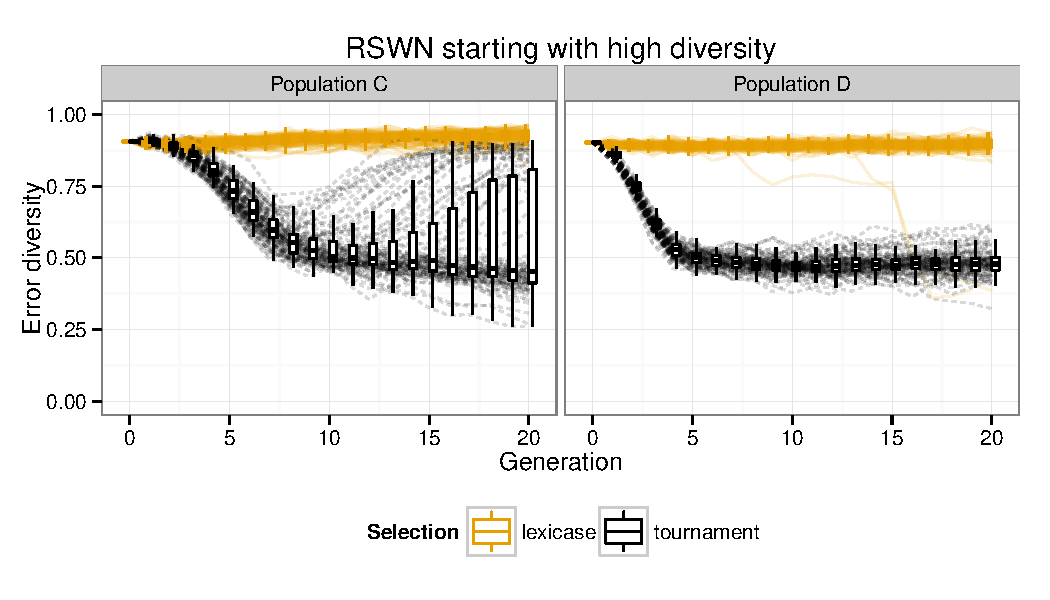
\includegraphics{../figures/RSWN_high_diversity}
	\vspace{-1 cm}
	\caption{Changes in diversity over 100 ``re-runs'' of the replace-space-with-newline problem with both lexicase and tournament selections, starting from a population with high diversity coming from a lexicase selection run.}
	\label{fig:RSWNhighDiversity}
\end{figure*}

\begin{figure*}
	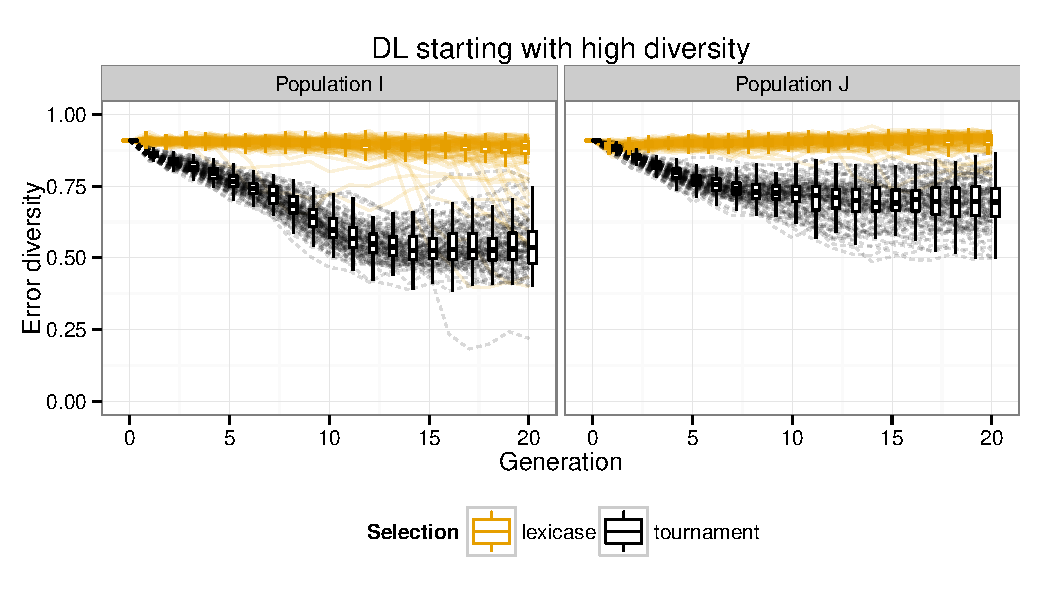
\includegraphics{../figures/DL_high_diversity}
	\vspace{-1 cm}
	\caption{Changes in diversity over 100 ``re-runs'' of the double-letters problem with both lexicase and tournament selections, starting from a population with high diversity coming from a lexicase selection run.}
	\label{fig:DLhighDiversity}
\end{figure*}

\subsection{Starting with low diversity}
\label{sec:lowDiversityResults}

\begin{figure*}
	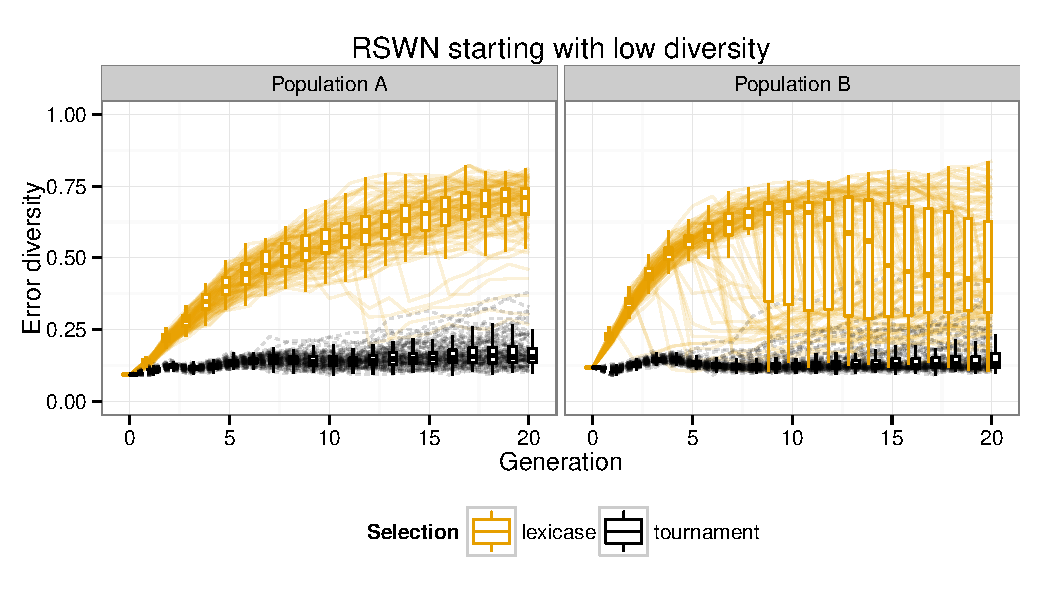
\includegraphics{../figures/RSWN_low_diversity}
	\vspace{-1 cm}
	\caption{Changes in diversity over 100 ``re-runs'' of the replace-space-with-newline problem with both lexicase and tournament selections, starting from a population with low diversity coming from a tournament selection run.}
	\label{fig:RSWNlowDiversity}
\end{figure*}

\begin{figure*}
	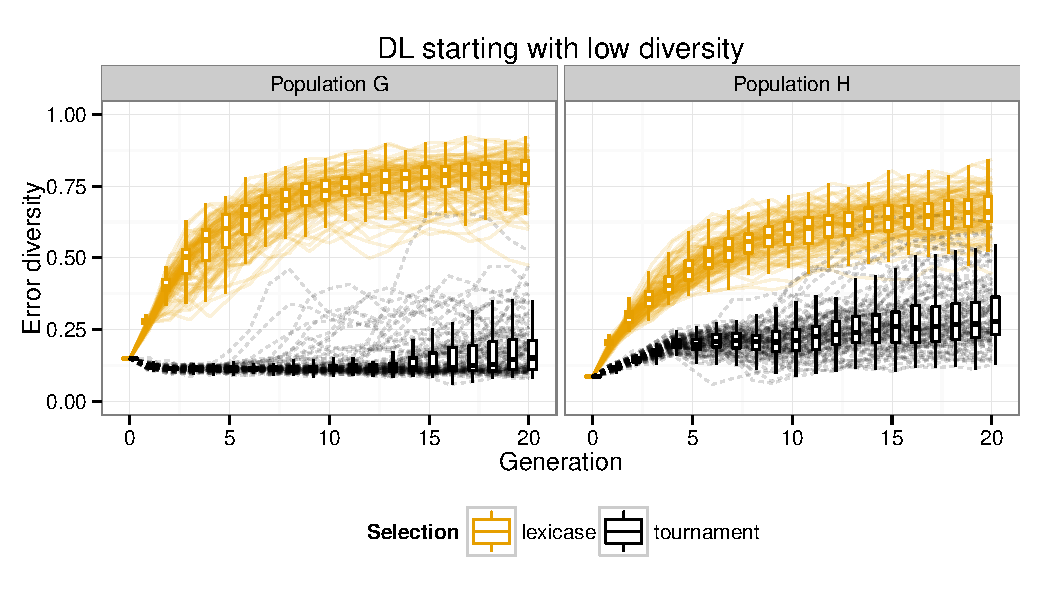
\includegraphics{../figures/DL_low_diversity}
	\vspace{-1 cm}
	\caption{Changes in diversity over 100 ``re-runs'' of the double-letters problem with both lexicase and tournament selections, starting from a population with low diversity coming from a tournament selection run.}
	\label{fig:DLlowDiversity}
\end{figure*}

\subsection{Starting after a diversity crash}
\label{sec:crashDiversityResults}

\begin{figure*}
	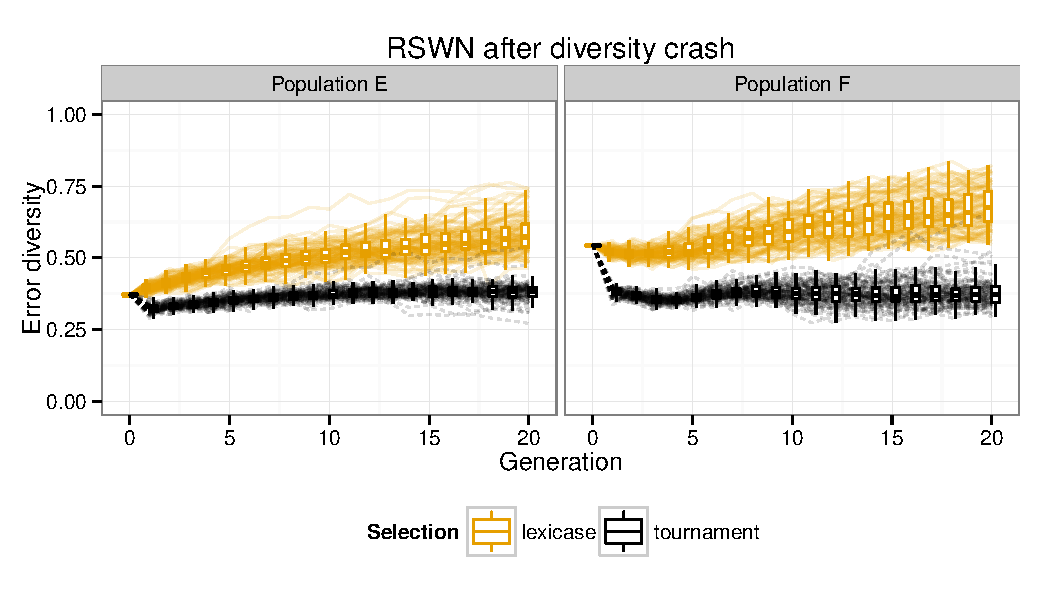
\includegraphics{../figures/RSWN_diversity_crash}
	\vspace{-1 cm}
	\caption{Changes in diversity over 100 ``re-runs'' of the replace-space-with-newline problem with both lexicase and tournament selections, starting from a population with that had lost diversity in a diversity crash in a lexicase selection run.}
	\label{fig:RSWNdiversityCrash}
\end{figure*}

\begin{figure*}
	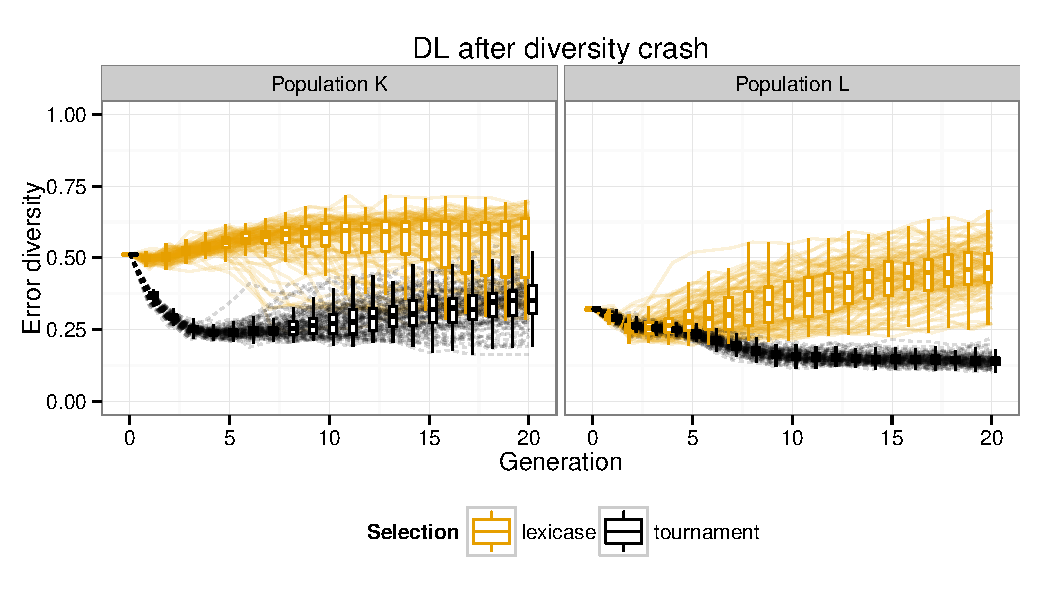
\includegraphics{../figures/DL_diversity_crash}
	\vspace{-1 cm}
	\caption{Changes in diversity over 100 ``re-runs'' of the double-letters problem with both lexicase and tournament selections, starting from a population with that had lost diversity in a diversity crash in a lexicase selection run.}
	\label{fig:DLdiversityCrash}
\end{figure*}


\section{Conclusions}
\label{sec:conclusions}

I'm hoping we have conclusions.

\section*{Acknowledgments}
Lots of cool people helped us.

% The following two commands are all you need in the
% initial runs of your .tex file to
% produce the bibliography for the citations in your paper.
\bibliographystyle{abbrv}
\bibliography{lexicase_recovery}  % sigproc.bib is the name of the Bibliography in this case
% You must have a proper ".bib" file
%  and remember to run:
% latex bibtex latex latex
% to resolve all references
%
% ACM needs 'a single self-contained file'!
%


% \balancecolumns % GM June 2007
\end{document}
